\documentclass[a4paper,justified,final,twoside,nobib]{tufte-book}

\hypersetup{colorlinks}% uncomment this line if you prefer colored hyperlinks (e.g., for onscreen viewing)

\usepackage{mathtools} %added mathtools for piecewise functions

%%
% Book metadata
\title{A\\Machine Learning\\Handbook\thanks{Thanks to Edward R.~Tufte for his inspiration.}}
\author[]{}
\publisher{Publisher of This Book}

%%
% Automated bibliography management
\usepackage{natbib}
\setcitestyle{authoryear}

%%
% If they're installed, use Bergamo and Chantilly from www.fontsite.com.
% They're clones of Bembo and Gill Sans, respectively.
%\IfFileExists{bergamo.sty}{\usepackage[osf]{bergamo}}{}% Bembo
%\IfFileExists{chantill.sty}{\usepackage{chantill}}{}% Gill Sans

\usepackage{microtype}

%%
% Describe algorithms using fancy pseudo code
\usepackage{algorithm}
\usepackage[noend]{algpseudocode}

%%
% Just some sample text
\usepackage{lipsum}
\usepackage{soul}
%%
% For nicely typeset tabular material
\usepackage{booktabs}
\usepackage{pdfpages}

%%
% For graphics / images
\usepackage{graphicx}
\setkeys{Gin}{width=\linewidth,totalheight=\textheight,keepaspectratio}
\graphicspath{{graphics/}}

% The fancyvrb package lets us customize the formatting of verbatim
% environments.  We use a slightly smaller font.
\usepackage{fancyvrb}
\fvset{fontsize=\normalsize}

%%
% Prints argument within hanging parentheses (i.e., parentheses that take
% up no horizontal space).  Useful in tabular environments.
\newcommand{\hangp}[1]{\makebox[0pt][r]{(}#1\makebox[0pt][l]{)}}

%%
% Prints an asterisk that takes up no horizontal space.
% Useful in tabular environments.
\newcommand{\hangstar}{\makebox[0pt][l]{*}}

%%
% Prints a trailing space in a smart way.
\usepackage{xspace}

%%
% Some shortcuts for Tufte's book titles.  The lowercase commands will
% produce the initials of the book title in italics.  The all-caps commands
% will print out the full title of the book in italics.
\newcommand{\vdqi}{\textit{VDQI}\xspace}
\newcommand{\ei}{\textit{EI}\xspace}
\newcommand{\ve}{\textit{VE}\xspace}
\newcommand{\be}{\textit{BE}\xspace}
\newcommand{\VDQI}{\textit{The Visual Display of Quantitative Information}\xspace}
\newcommand{\EI}{\textit{Envisioning Information}\xspace}
\newcommand{\VE}{\textit{Visual Explanations}\xspace}
\newcommand{\BE}{\textit{Beautiful Evidence}\xspace}
\newcommand{\ics}{\smallcaps{ICS5110 Applied Machine Learning\xspace}}

\newcommand{\TL}{Tufte-\LaTeX\xspace}

% Prints the month name (e.g., January) and the year (e.g., 2008)
\newcommand{\monthyear}{%
  \ifcase\month\or January\or February\or March\or April\or May\or June\or
  July\or August\or September\or October\or November\or
  December\fi\space\number\year
}

% Prints an epigraph and speaker in sans serif, all-caps type.
\newcommand{\openepigraph}[2]{%
  %\sffamily\fontsize{14}{16}\selectfont
  \begin{fullwidth}
  \sffamily\large
  \begin{doublespace}
  \noindent\allcaps{#1}\\% epigraph
  \noindent\allcaps{#2}% author
  \end{doublespace}
  \end{fullwidth}
}

% Inserts a blank page
\newcommand{\blankpage}{\newpage\hbox{}\thispagestyle{empty}\newpage}

\usepackage{units}

% Typesets the font size, leading, and measure in the form of 10/12x26 pc.
\newcommand{\measure}[3]{#1/#2$\times$\unit[#3]{pc}}

% Macros for typesetting the documentation
\newcommand{\hlred}[1]{\textcolor{Maroon}{#1}}% prints in red
\newcommand{\hangleft}[1]{\makebox[0pt][r]{#1}}
\newcommand{\hairsp}{\hspace{1pt}}% hair space
\newcommand{\hquad}{\hskip0.5em\relax}% half quad space
\newcommand{\TODO}{\textcolor{red}{\bf TODO!}\xspace}
\newcommand{\ie}{\textit{i.\hairsp{}e.}\xspace}
\newcommand{\eg}{\textit{e.\hairsp{}g.}\xspace}
\newcommand{\na}{\quad--}% used in tables for N/A cells
\providecommand{\XeLaTeX}{X\lower.5ex\hbox{\kern-0.15em\reflectbox{E}}\kern-0.1em\LaTeX}
\newcommand{\tXeLaTeX}{\XeLaTeX\index{XeLaTeX@\protect\XeLaTeX}}
% \index{\texttt{\textbackslash xyz}@\hangleft{\texttt{\textbackslash}}\texttt{xyz}}
\newcommand{\tuftebs}{\symbol{'134}}% a backslash in tt type in OT1/T1
\newcommand{\doccmdnoindex}[2][]{\texttt{\tuftebs#2}}% command name -- adds backslash automatically (and doesn't add cmd to the index)
\newcommand{\doccmddef}[2][]{%
  \hlred{\texttt{\tuftebs#2}}\label{cmd:#2}%
  \ifthenelse{\isempty{#1}}%
    {% add the command to the index
      \index{#2 command@\protect\hangleft{\texttt{\tuftebs}}\texttt{#2}}% command name
    }%
    {% add the command and package to the index
      \index{#2 command@\protect\hangleft{\texttt{\tuftebs}}\texttt{#2} (\texttt{#1} package)}% command name
      \index{#1 package@\texttt{#1} package}\index{packages!#1@\texttt{#1}}% package name
    }%
}% command name -- adds backslash automatically
\newcommand{\doccmd}[2][]{%
  \texttt{\tuftebs#2}%
  \ifthenelse{\isempty{#1}}%
    {% add the command to the index
      \index{#2 command@\protect\hangleft{\texttt{\tuftebs}}\texttt{#2}}% command name
    }%
    {% add the command and package to the index
      \index{#2 command@\protect\hangleft{\texttt{\tuftebs}}\texttt{#2} (\texttt{#1} package)}% command name
      \index{#1 package@\texttt{#1} package}\index{packages!#1@\texttt{#1}}% package name
    }%
}% command name -- adds backslash automatically
\newcommand{\docopt}[1]{\ensuremath{\langle}\textrm{\textit{#1}}\ensuremath{\rangle}}% optional command argument
\newcommand{\docarg}[1]{\textrm{\textit{#1}}}% (required) command argument
\newenvironment{docspec}{\begin{quotation}\ttfamily\parskip0pt\parindent0pt\ignorespaces}{\end{quotation}}% command specification environment
\newcommand{\docenv}[1]{\texttt{#1}\index{#1 environment@\texttt{#1} environment}\index{environments!#1@\texttt{#1}}}% environment name
\newcommand{\docenvdef}[1]{\hlred{\texttt{#1}}\label{env:#1}\index{#1 environment@\texttt{#1} environment}\index{environments!#1@\texttt{#1}}}% environment name
\newcommand{\docpkg}[1]{\texttt{#1}\index{#1 package@\texttt{#1} package}\index{packages!#1@\texttt{#1}}}% package name
\newcommand{\doccls}[1]{\texttt{#1}}% document class name
\newcommand{\docclsopt}[1]{\texttt{#1}\index{#1 class option@\texttt{#1} class option}\index{class options!#1@\texttt{#1}}}% document class option name
\newcommand{\docclsoptdef}[1]{\hlred{\texttt{#1}}\label{clsopt:#1}\index{#1 class option@\texttt{#1} class option}\index{class options!#1@\texttt{#1}}}% document class option name defined
\newcommand{\docmsg}[2]{\bigskip\begin{fullwidth}\noindent\ttfamily#1\end{fullwidth}\medskip\par\noindent#2}
\newcommand{\docfilehook}[2]{\texttt{#1}\index{file hooks!#2}\index{#1@\texttt{#1}}}
\newcommand{\doccounter}[1]{\texttt{#1}\index{#1 counter@\texttt{#1} counter}}

% Generates the index
\usepackage{makeidx}
\makeindex

\usepackage{tikz}

\begin{document}
%% Cover Page
\begingroup
\thispagestyle{empty}
\begin{tikzpicture}[remember picture,overlay]
\node[inner sep=0pt, outer sep=0pt] (background) at (current page.center) {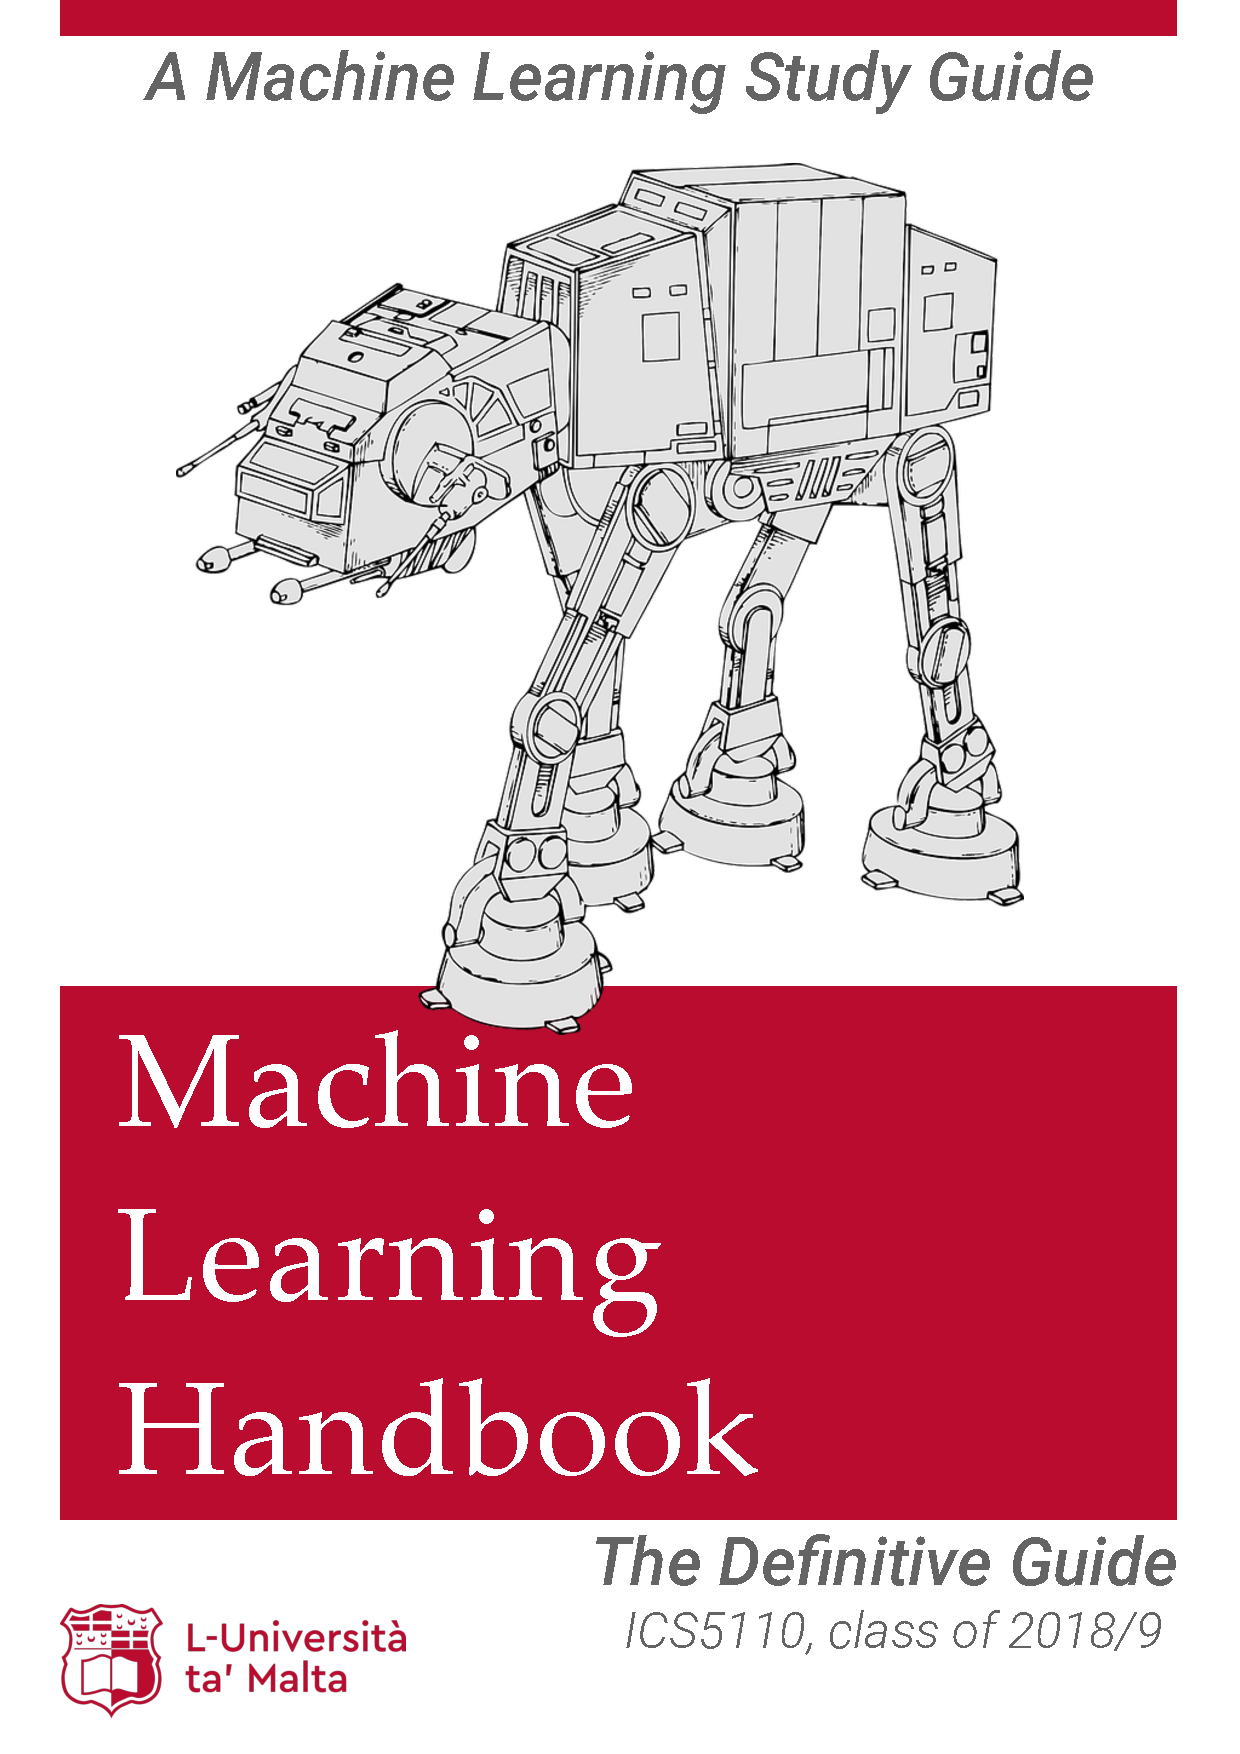
\includegraphics[width=\paperwidth]{cover/cover_oreilly_style.pdf}};
\end{tikzpicture}
\vfill
\endgroup

% Front matter
\frontmatter

% r.3 full title page
%% \maketitle


% v.4 copyright page
\newpage
\begin{fullwidth}
~\vfill
\thispagestyle{empty}
\setlength{\parindent}{0pt}
\setlength{\parskip}{\baselineskip}
\begin{figure*}[h]
	
\includegraphics[width=2.5in]{UMLOGO_redRGB.png}%
\end{figure*}

\par Copyright \copyright\ \the\year\ \ics\ class of 2018/9, University of Malta.

\par\smallcaps{Jean-Paul Ebejer, Dylan Seychell, Lara Marie Demajo, Daniel Farrugia, Keith Mintoff, David Farrugia, Ivan Salomone \hl{ADD YOUR NAME TO THIS LIST}} %TODO

\par Licensed under the Apache License, Version 2.0 (the ``License''); you may not
use this file except in compliance with the License. You may obtain a copy
of the License at \url{http://www.apache.org/licenses/LICENSE-2.0}. Unless
required by applicable law or agreed to in writing, software distributed
under the License is distributed on an \smallcaps{``AS IS'' BASIS, WITHOUT
WARRANTIES OR CONDITIONS OF ANY KIND}, either express or implied. See the
License for the specific language governing permissions and limitations
under the License.\index{license}

\par\textit{First printing, \monthyear}
\end{fullwidth}

% r.5 contents
\tableofcontents

%%\listoffigures

%%\listoftables

% r.9 introduction
\cleardoublepage
\chapter{Introduction}

This book explains popular Machine Learning terms.  We focus to explain each term comprehensively, through the use of examples and diagrams.  The description of each term is written by a student sitting in for \ics\footnote{\url{https://www.um.edu.mt/courses/studyunit/ICS5110}} at the University of Malta (class 2018/2019).  This study-unit is part of the MSc.\ in AI offered by the Department of Artificial Intelligence, Faculty of ICT.

%%
% Start the main matter (normal chapters)
\mainmatter

%% JP's example file -- file must be stored in directory "terms" and have
%% the term and initials of the student in the filename.
\chapter[Activation Functions]{Activation Functions}
\label{ch:activation-functions}\index{activation functions|(}
\citet{caterini2018} defined artificial neural networks as ``a model that would imitate the function of the human brain---a set of neurons joined together by a set of connections. Neurons, in this context, are composed of a weighted sum of their inputs followed by a nonlinear function, which is also known as an activation function.''

Activation functions are used in artificial neural networks to determine whether the output of the neuron should be considered further or ignored. If the activation function chooses to continue considering the output of a neuron, we say that the neuron has been activated. The output of the activation function is what is passed on to the subsequent layer in a multilayer neural network. To determine whether a neuron should be activated, the activation function takes the output of a neuron and transforms it into a value commonly bound to a specific range, typically from 0 to 1 or -1 to 1 depending on the which activation function is applied.

\section{Step Function}\label{sec:step-function}\index{activation functions!step function}

\begin{marginfigure}
  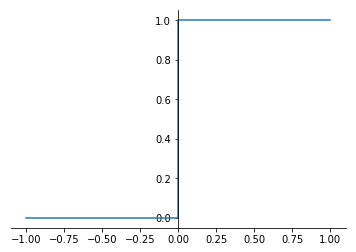
\includegraphics{graphics/activation_functions/step_function.png}
  \caption{
    A graph of the step function. 
  }
  \label{fig:stepfunction}
\end{marginfigure}

\begin{equation}\label{stepfunction}
    f(x) =
    \begin{dcases*}
        0 & \text{for \(x < 0\)} \\
        1 & \text{for \(x \geq 0\)} \\
    \end{dcases*}
\end{equation}

\begin{equation}\label{stepfunctionderivative}
    \frac{d}{d(x)}f(x) =
      \begin{dcases*}
                                       0 & \text{for \(x \neq 0\)} \\
                                       ? & \text{for \(x = 0\)} \\
      \end{dcases*}
\end{equation}

The Heavside step function, visualised in figure~\ref{fig:stepfunction} and defined by equation~\ref{stepfunction}, is one of the simplest activation functions that can be used in a neural network. This function returns 0 if the input of a node is less than a predetermined threshold (typically 0), or otherwise it returns 1 if the output of the node is greater than or equal to the threshold. This activation function was first used in a machine learning context by \citet{rosenblatt1957perceptron} in his seminal work describing the perceptron, the precursor to the modern day neural network. 

Nowadays, the step function is seldom used in practice as it cannot be used to classify more than one class. Furthermore, since the derivative of this function is 0 , as defined by equation~\ref{stepfunctionderivative}, gradient descent algorithms are not be able to progressively update the weights of a network that makes use of this function \citep{Snyman2005}.

\section{Linear Functions}\label{sec:linear-function}\index{activation functions!linear activation function}

\begin{equation}\label{linearfunction}
    f(x) = ax + b
\end{equation}

\begin{equation}\label{linearfunctionderivative}
    \frac{d}{d(x)}f(x) = a
\end{equation}

A linear activation function, is any function in the format of equation~\ref{linearfunction}, where $a, b \in \mathbb{R}$. This function seeks to solve some of the shortcomings of the step function. The output produced by a linear activation function is proportional to the input. This property means that linear activation functions can be used for multi-class problems. However, linear functions can only be utilised on problems that are linearly separable and can also run into problems with gradient descent algorithms, as the derivative of a linear function is a constant, as seen in equation~\ref{linearfunctionderivative}. Additionally, since the output of the linear function is not bound to any range, it could be susceptible to a common problem when training deep neural networks called the exploding gradient problem, which can make learning unstable \citep{goodfellow2016deeplearning}.

\section{Sigmoid Function}\label{sec:sigmoid}\index{activation functions!sigmoid function}

\begin{marginfigure}
  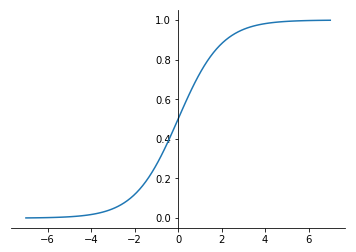
\includegraphics{graphics/activation_functions/sigmoid_function.png}
  \caption{
    A graph of the sigmoid function.
  }
  \label{fig:sigmoidfunction}
\end{marginfigure}

\begin{equation}\label{sigmoidfunction}
    f(x) = \frac{1}{(1 + e^{-x})}
\end{equation}

\begin{equation}\label{sigmoidfunctionderivative}
    \frac{d}{d(x)}f(x) = f(x)(1-f(x))
\end{equation}

The sigmoid function or logistic function, visualised in figure~\ref{fig:sigmoidfunction} and represented by  equation~\ref{sigmoidfunction}, is one of the most commonly used activation functions in neural networks, because of its simplicity and desirable properties. The use of this function in neural networks was first introduced by \citet{DavidE.Rumelhart1986Lrbb}, in one of the most important papers in the field of machine learning, which described the back-propagation algorithm and the introduction of hidden layers, giving rise to modern day neural networks.  The values produced by the sigmoid function are bound between 0 and 1, both not inclusive, which help manage the exploding gradient problem. The derivative of this function, represented by equation~\ref{sigmoidfunctionderivative}, produces a very steep gradient for a relatively small range of values, typically in the range of $-2$ to $2$. This means that for most inputs that the function receives it will return values that are very close to either 0 or 1.

On the other hand, this last property makes the sigmoid function very susceptible to the vanishing gradient problem \citep{bengio94}. When observing the shape of the sigmoid function we see that towards the ends of the curve, the function becomes very unresponsive to changes in the input. In other words, the gradient of the function for large inputs becomes very close to 0. This can become very problematic for neural networks that are very deep in design, such as recurrent neural networks (RNNs).To address this problems in RNNs Long Short-Term Memory (LSTM) units where introduced as a variant of the traditional RNN architecture \citep{hochreiter1997long}.

\section{Hyperbolic Tangent}\label{sec:tanh}\index{activation functions!hyperbolic tangent}
\begin{marginfigure}
  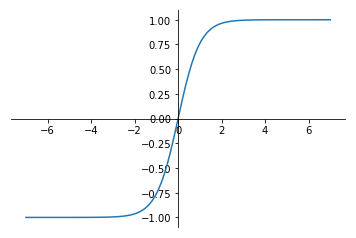
\includegraphics{graphics/activation_functions/tanh_function.png}
  \caption{
    A graph of the hyperbolic tangent (tanh) function.
  }
  \label{fig:tanhfunction}
\end{marginfigure}

\begin{equation}\label{tanhfunction}
    f(x) = \frac{(e^{x} - e^{-x})}{(e^{x} + e^{-x})}
\end{equation}

\begin{equation}\label{tanhfunctionderivative}
    \frac{d}{d(x)}f(x) = 1-f(x)^2.
\end{equation}

The hyperbolic tangent (tanh) function, visualised in figure~\ref{fig:tanhfunction} and represented by equation~\ref{tanhfunction}, is another common activation function that is sometimes used instead of sigmoid. The tanh function has the same characteristics of the sigmoid function mentioned above. In fact, when comparing figure~\ref{fig:sigmoidfunction} to figure~\ref{fig:tanhfunction} one can observe that the tanh function is simply a scaled and translated version of the sigmoid function. As a result of this scaling and translation, the tanh function has a steeper gradient towards the origin, and it returns values between -1 and 1. The derivative of the hyperbolic tangent function is represented by equation~\ref{tanhfunctionderivative}.

\citet{lecun2012efficient} analysed various factors that affect the performance of backpropagation, and suggested that tanh may be better suited than sigmoid as an activation function due to its symmetry about the origin, which is more likely to produce outputs that are on average close to zero, resulting in sparser activations. This means that not all nodes in the network need to be computed, leading to better performance. \citet{glorot2010understanding} studied in detail the effects of the sigmoid and tanh activation functions and noted how the sigmoid function in particular is not well suited for deep networks with random initialisation and go on to propose an alternative normalised initialisation scheme which produced better performance in their experiments.

\section{Rectified Linear Unit}\label{sec:relu}\index{activation functions!rectified linear unit (relu)}
\begin{marginfigure}
  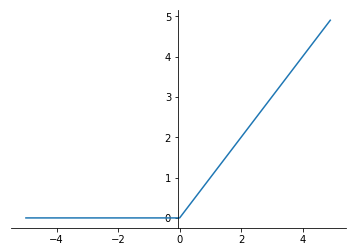
\includegraphics{graphics/activation_functions/relu_function.png}
  \caption{
    A graph of the ReLU function.
  }
  \label{fig:relugraph}
\end{marginfigure}

\begin{equation}\label{relufunction}
    f(x) =
      \begin{dcases*}
                                       0 & \text{for $x < 0$} \\
                                       x & \text{for $x \geq 0$} \\
      \end{dcases*}
\end{equation}

\begin{equation}\label{relufunctionderivative}
    \frac{d}{d(x)}f(x) =
      \begin{dcases*}
                                       0 & \text{for $x < 0$} \\
                                       1 & \text{for $x \geq 0$} \\
      \end{dcases*}
\end{equation}

The Rectified Linear Unit (ReLU) function, visualised in figure~\ref{fig:relugraph} and represented by  equation~\ref{relufunction}, returns 0 if the input of the function is negative, otherwise it outputs the value of the input itself. This function is non-linear in nature even though at first glance it may seem similar to an identity function. The ReLU function is becoming one of the more commonly used activation functions due to its simplicity, performance, and suitability to networks with many layers. Another benefit of the ReLU function is that it produces sparse activations unlike many other commonly used functions such as the sigmoid. 

The ReLU function has been used in many neural network models to improve their performance. \citet{Nair2010} use ReLU to improve the performance of Restricted Boltzmann Machines in object recognition. \citet{KrizhevskyAlex2017Icwd} introduced a breakthrough Convolutional Neural Network (CNN) architecture called AlexNet, which pioneered the use of the ReLU activation function together with dropout layers to minimise over fitting in CNNs. 

Unfortunately, because the gradient of the function for inputs that are negative is 0, as seen in equation~\ref{relufunctionderivative}, the ReLU function can still be susceptible to the vanishing gradient problem. To manage this problem a variant of the ReLU function, called Leaky ReLU is sometimes used. Rather than simply returning 0 for negative inputs, the leaky ReLU returns a very small value such as $0.01x$. \citet{maas2013rectifier} compared the performance of Sigmoid, ReLU and Leaky ReLU functions and found that while the the performance of both the ReLU and Leaky ReLU functions was better than the performance achieved with the sigmoid function, the performance of the two ReLU functions was nearly identical.
\index{activation functions|)}

\chapter{Confusion Matrix}
\label{ch:confusion-matrix}\index{confusion matrix|(}

A \textit{Confusion Matrix} (CM), is a contingency table showing how well a model classifies categorical data. By convention \citep{sammut2017encyclopedia}, the CM of an N-class model is an N$\times$N matrix indexed by the true class in the row dimension and the predicted class in the column dimension (Table~\ref{tab:cm_spam}).

\begin{table}[ht]
  \centering
  \fontfamily{ppl}\selectfont
  \begin{tabular}{llll}
    \toprule
                        &                     & \multicolumn{2}{c}{\textbf{Predicted Class}} \\
                        &                     & \textit{spam} & \textit{$\neg$spam} \\
    \midrule
    \textbf{True Class} & \textit{spam}       & 10           & 1 \\
                        & \textit{$\neg$spam} & 2            & 100 \\
    \bottomrule
  \end{tabular}
  \caption{CM of a hypothetical binary classifier which predicts whether out-of-sample text objects are spam or not. In this example, 10 spam and 100 non-spam objects are classified correctly, whilst 1 spam and 2 non-spam objects are misclassified.}
  \label{tab:cm_spam}
\end{table}
\vspace{2mm}

Even though CMs are commonly used to evaluate binary classifiers, they are not restricted to 2-class models \citep{martin2018speech}. A CM of a multi-class model would show the number of times the classes were predicted correctly and which classes were confused with each other (Table~\ref{tab:cm_sweets}).

\begin{table}[ht]
  \centering
  \fontfamily{ppl}\selectfont
  \begin{tabular}{llll}
    \toprule
                      & \textit{M\&M's} & \textit{Skittles} & \textit{Smarties} \\
    \midrule
    \textit{M\&M's}   & 34              & 3                 & 8  \\
    \textit{Skittles} & 1               & 28                & 5  \\
    \textit{Smarties} & 2               & 4                 & 22 \\
    \bottomrule
  \end{tabular}
  \caption{CM of a hypothetical sweets classifier. The main diagonal of the CM shows the number of correct predictions, whilst the remaining elements indicate how many sweets were misclassified.}
  \label{tab:cm_sweets}
\end{table}
\vspace{2mm}

The CM of the model $h : X \mapsto C$ over the concept $c : X \mapsto C$ using dataset $S \subset X$ is formally defined  as a matrix $\Xi$ such that $\Xi_{c,S}(h)[d_1,d_2] = |S_{h=d_1,c=d_2}|$ \citep{cichosz2014data}. The CM is constructed by incrementing the element corresponding to the true class \textit{vis-a-vis} the predicted class for each object in the dataset (Algorithm \ref{alg:cm}).

\begin{algorithm}
  \begin{algorithmic}
    \State $\Xi \gets 0$
    \For{$x \in S$}
      \State $d_1 \gets c(x)$
      \State $d_2 \gets h(x)$
      \State $\Xi_{d_1,d_2} \gets \Xi_{d_1,d_2} + 1$
    \EndFor
  \end{algorithmic}
  \caption{The CM is initialised to the zero matrix, and populated by iterating over all the objects $x$ with corresponding true class $d_1$ and predicted class $d_2$ and incrementing the element $(d_1,d_2)$ by 1 for each matching outcome.}
  \label{alg:cm}
\end{algorithm}

In binary classification, the CM consists of 2 specially designated classes called the \textit{positive} class and the \textit{negative} class \citep{saito2015precision}. As indicated in Table~\ref{tab:cm_binary}, positive outcomes from the true class  which are classified correctly are called \textit{True Positives}\index{true positives} (TP), whilst misclassifications are called \textit{False Negatives}\index{false negatives} (FN). On the other hand, negative true class outcomes which are classified correctly are called \textit{True Negatives}\index{true negatives} (TN), and misclassifications are called \textit{False Positives}\index{false positives} (FP). In natural sciences, FP are called \textit{Type I Errors} and FN are known as \textit{Type II Errors} \citep{fielding1997review}.

\begin{table}[ht]
  \centering
  \fontfamily{ppl}\selectfont
  \begin{tabular}{lll}
    \toprule
                  & \textit{+ve} & \textit{-ve} \\
    \midrule
    \textit{+ve}  & TP           & FN \\
    \textit{-ve}  & FP           & TN \\
    \bottomrule
  \end{tabular}
  \caption{CMs of binary classifiers have positive (+ve) and negative (-ve) classes, and elements called \textit{True Positives} (TP), \textit{False Positives} (FP), \textit{True Negatives} (TN) and \textit{False Negatives} (FN).}
  \label{tab:cm_binary}
\end{table}
\vspace{2mm}

The information presented in the CM can be used to evaluate the performance of different binary classifiers \citep{lu2004predicting}. A number of statistics (Equations~\ref{eq:cm_acc}-\ref{eq:cm_fscore}) derived from the CM have been proposed in the literature \citep{deng2016improved} to gain a better understanding of what are the strengths and weaknesses of different classifiers. Caution should be exercised when interpreting metrics \citep{jeni2013facing}, since the CM could be misleading if the data is imbalanced and an important subrange of the domain is underrepresented \citep{raeder2012learning}. For instance, an albino zebra classifier which always returns negative will achieve high accuracy since albinism is a rare disorder.

These metrics are important in situations in which a particular type of misclassification, i.e. FP or FN, could have worse consequences than the other \citep{hassanien2017advances}. For example, FP are more tolerable than FN in classifiers which predict whether a patient has a disease. Both outcomes are undesirable, but in medical applications it is better to err on the side of caution since FN could be fatal.

\textit{Accuracy}\index{confusion matrix!accuracy} (ACC) is the proportion of correct predictions (Equation~\ref{eq:cm_acc}). It is a class-insensitive metric because it can give a high rating to a model which classifies majority class objects correctly but misclassifies interesting minority class objects \citep{branco2016survey}. The other metrics should be preferred since they are more class-sensitive and give better indicators when the dataset is imbalanced.

\begin{equation}
\label{eq:cm_acc}
ACC = \frac{|TP \cup TN|}{|TP \cup FP \cup TN \cup FN|}
\end{equation}

\textit{Negative Predictive Value}\index{confusion matrix!negative predictive value} (NPV) is the ratio of the correct negative predictions from the total negative predictions (Equation~\ref{eq:cm_npv}).

\begin{equation}
\label{eq:cm_npv}
NPV = \frac{|TN|}{|TN \cup FN|}
\end{equation}

\textit{True Negative Rate}\index{confusion matrix!true negative rate} (TNR), or \textit{Specificity}\index{confusion matrix!true negative rate!specificity}, is the ratio of the correct negative predictions from the total true negatives (Equation~\ref{eq:cm_tnr}).

\begin{equation}
\label{eq:cm_tnr}
TNR = \frac{|TN|}{|TN \cup FP|}
\end{equation}

\textit{True Positive Rate}\index{confusion matrix!true positive rate} (TPR), also called \textit{Sensitivity}\index{confusion matrix!true positive rate!sensitivity} or \textit{Recall}\index{confusion matrix!true positive rate!recall}, is the ratio of the correct positive predictions from the total true positives (Equation~\ref{eq:cm_tpr}).

\begin{equation}
\label{eq:cm_tpr}
TPR = \frac{|TP|}{|TP \cup FN|}
\end{equation}

Sensitivity and Specificity can be combined into a single metric (Equation~\ref{eq:cm_ss}). These metrics are often used in  domains in which minority classes are important \citep{kuhn2013applied}. For example, the Sensitivity of a medical classifier \citep{el2010hybrid} measures how many patients with the condition tested positive, and Specificity measures how many did not have the condition and tested negative.

\begin{equation}
\label{eq:cm_ss}
\textnormal{\textit{Sensitivity}} \times \textnormal{\textit{Specificity}} = \frac{|TP| \times |TN|}{|TP \cup FN| \times |TN \cup FP|}
\end{equation}

\textit{Positive Predictive Value}\index{confusion matrix!positive predictive value} (PPV), or \textit{Precision}\index{confusion matrix!positive predictive value!precision}, is the ratio of the correct positive predictions from the total positive predictions (Equation~\ref{eq:cm_ppv}). The difference between accuracy and precision is depicted in Figure~\ref{fig:cm_accprec}.

\begin{equation}
\label{eq:cm_ppv}
PPV = \frac{|TP|}{|TP \cup FP|}
\end{equation}

\begin{marginfigure}
  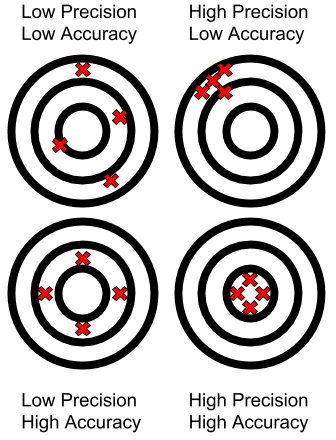
\includegraphics{confusion_matrix/accprec.png}
  \caption{Accuracy vs Precision.}
  \label{fig:cm_accprec}
\end{marginfigure}

Precision and Recall are borrowed from the discipline of \textit{Information Extraction} \citep{sokolova2009systematic}. A composite metric called \textit{F-score}\index{confusion matrix!f-score}, \textit{F1-score}\index{confusion matrix!f-score!f1-score}, or \textit{F-measure}\index{confusion matrix!f-score!f-measure} (Equation~\ref{eq:cm_fscore}) can be derived by finding their harmonic mean \citep{kelleher2015fundamentals}.

\begin{equation}
\label{eq:cm_fscore}
\textnormal{\textit{F-score}} = 2 \times \frac{PPV \times TPR}{PPV + TPR}
\end{equation}

The complements of ACC, NPV, TNR, TPR and PPV are called, respectively, \textit{Error Rate}\index{confusion matrix!error rate}, \textit{False Omission Rate}\index{confusion matrix!false omission rate}, \textit{false positive rate}\index{confusion matrix!false positive rate}, \textit{false negative rate}\index{confusion matrix!false negative rate} and \textit{False Discovery Rate}\index{confusion matrix!false discovery rate}.

The metrics can be adapted for evaluating multi-class models by decomposing an N-class CM into 2-class CMs, and evaluating them individually \citep{stager2006dealing}. The literature describes two methods for decomposing this kind of  CM. In the \textit{1-vs-1}\index{confusion matrix!1-vs-1} approach, 2-class CMs are constructed for each pairwise class as shown in Table~\ref{tab:cm_1vs1}.

\begin{table}[ht]
  \centering
  \fontfamily{ppl}\selectfont
  \begin{tabular}{ll}
    \toprule
    \textit{+ve} & \textit{-ve} \\
    \midrule
    M\&M's       & $\{$Skittles, Smarties$\}$ \\
    Skittles     & $\{$M\&M's, Smarties$\}$ \\
    Smarties     & $\{$M\&M's, Skittles$\}$ \\
    \bottomrule
  \end{tabular}
  \caption{2-class CMs derived from the classes in Table~\ref{tab:cm_sweets}. The +ve classes are paired separately with each -ve class.}
  \label{tab:cm_1vs1}
\end{table}
\vspace{2mm}

In the \textit{1-vs-rest}\index{confusion matrix!1-vs-rest} approach, 2-class CMs are constructed for each class and the remaining classes combined together as shown in Table~\ref{tab:cm_1vsN}.

\begin{table}[ht]
  \centering
  \fontfamily{ppl}\selectfont
  \begin{tabular}{ll}
    \toprule
    +ve       & -ve \\
    \midrule
    M\&M's    & Skittles $\cup$ Smarties \\
    Skittles  & M\&M's $\cup$ Smarties \\
    Smarties  & Skittles $\cup$ M\&M's \\
    \bottomrule
  \end{tabular}
  \caption{2-class CMs derived through decomposition of the 3-class CM from Table~\ref{tab:cm_sweets} using the 1-vs-rest approach.}
  \label{tab:cm_1vsN}
\end{table}
\vspace{2mm}

Using all metrics could be counterproductive due to information redundancy, but none of the metrics is enough on its own \citep{ma2007adequate}. For instance, Recall is class-sensitive but it would give a perfect score to an inept model which simply returns the positive class. Thus, the best approach is to evaluate with complementary pairs \citep{gu2009evaluation} such as Sensitivity \textit{vs} Specificity, or Precision \textit{vs} Recall; or a combined measure such as the F-score.

Taking into account the above, CMs are suitable for visualising, evaluating, and comparing the performance of binary or multi-class classifiers. They should be used in conjunction with metrics such as the F-measure to avoid bias, especially if the dataset is unbalanced. For further details on the theoretical aspects of CMs and for practical examples in R refer to \citep{cichosz2014data}; for examples in Python refer to \citep{muller2016introduction}.

The following example is motivated by the samples in the \textit{Scikit-Learn} documentation and the work of  \citep{geron2017hands}. The models in Figure~\ref{fig:cm_model} were trained on the \textit{wines} dataset included with Scikit-Learn.

\begin{figure}
  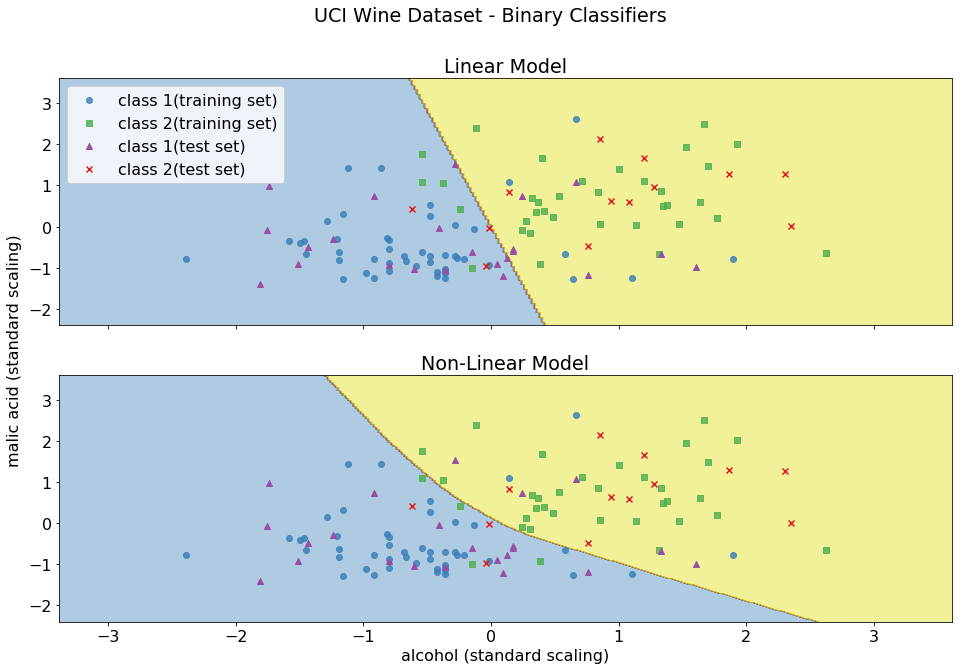
\includegraphics{confusion_matrix/model.png}
  \caption{Decision boundary learned by a linear and non-linear binary classifier.}
  \label{fig:cm_model}
\end{figure}

\begin{margintable}
  \begin{tabular}{lll}
    \toprule
                 & Linear & Non-Linear \\
    \midrule
    Accuracy     & 0.72   & 0.78 \\
    Specificity  & 0.77   & 0.77 \\
    Sensitivity  & 0.70   & 0.78 \\
    Precision    & 0.84   & 0.86 \\
    F-score      & 0.76   & 0.82 \\
    \bottomrule
  \end{tabular}
  \caption{Statistics derived from the CMs in Figure~\ref{fig:cm_wines}.}
  \label{tab:cm_metrics}
\end{margintable}

As it can be intuitively deduced from Figure~\ref{fig:cm_model}, the decision boundary of the non-linear model is a better fit than the linear model. The CMs in Figure~\ref{fig:cm_wines} also show that non-linear model performs better with a higher TP, and consequently lower TN. The biggest advantage of the non-linear model is the higher Sensitivity resulting in a better F-score.

\begin{figure}
  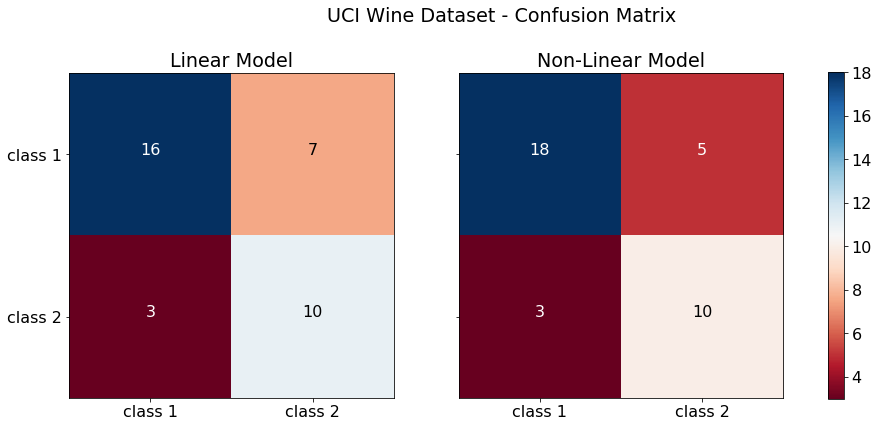
\includegraphics{confusion_matrix/cm.png}
  \caption{The linear classifier has 16 TP, 10 TN, 7 FN and 3 FP, whilst the non-linear classifier has 18 TP, 10 TN, 5 FN and 3 FP.}
  \label{fig:cm_wines}
\end{figure}

\index{confusion matrix|)}
\chapter{\textit{}Cross-Validation}
\label{ch:cross-validation}\index{cross-validation}

Cross-validation (CV) is an estimation method used on supervised learning algorithms to assess their ability to predict the output of unseen data \cite[-3\baselineskip]{varma2006bias,kohavi1995study}. Supervised learning algorithms are computational tasks like classification or regression, that learn an input-output function based on a set of samples. Such samples are also known as the labeled training data where each example consists of an input vector and its correct output value. After the training phase, a supervised learning algorithm should be able to use the inferred function in order to map new input unseen instances, known as testing data, to their correct output values \cite{caruana2006empirical}. When the algorithm incorporates supervised feature selection, cross-validation should always be done external to the selection (feature-selection performed within every CV iteration) so as to ensure the test data remains unseen, reducing bias \cite[-3\baselineskip]{ambroise2002selection, friedman2001elements}.  Therefore, cross-validation, also known as out-of-sample testing, tests the function's ability to generalize to unseen situations \cite[-3\baselineskip]{varma2006bias,kohavi1995study}. 

Cross-validation has two types of approaches, being i) the exhaustive cross validation approach which divides all the original samples in every possible way, forming training and test sets to train and test the model, and ii) the non-exhaustive cross validation approach which does not consider all the possible ways of splitting the original samples \cite{arlot2010survey}. Each of these approaches are further divided into different cross-validation methods, which are explained below.
\\\\
\noindent\textbf{Exhaustive cross-validation}
\begin{itemize}
\item Leave-$p$-out (L$p$O) \newline \index{leave-p-out}
This method takes $p$ samples from the data set as the test set and keeps the remaining as the training set, as shown in Fig.~\ref{fig:leavep}a. This is repeated for every combination of test and training set formed from the original data set and the average error is obtained. Therefore, this method trains and tests the algorithm $n\choose p$ times when the number of samples in the original data set is $n$, becoming inapplicable when $p>1$ \cite{arlot2010survey}.

\item Leave-one-out (LOO)\newline \index{leave-one-out}
This method is a specific case of the LpO method having $p=1$. It requires less computation efforts than LpO since the process is only repeated $n choose 1$ $= n$ times, however might still be inapplicable for large values of $n$ \cite{arlot2010survey}. 
\end{itemize}

\begin{figure*}
\centering
\begin{subfigure}
  \centering
  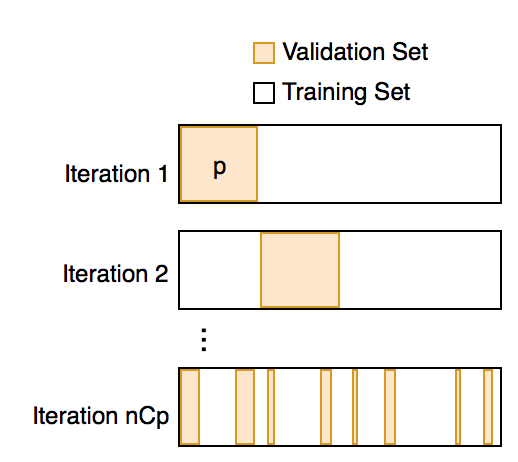
\includegraphics[width=.4\linewidth]{leavep.png}
  \caption{Leave-p-Out}
  \end{subfigure}
 \begin{subfigure}
  \centering
  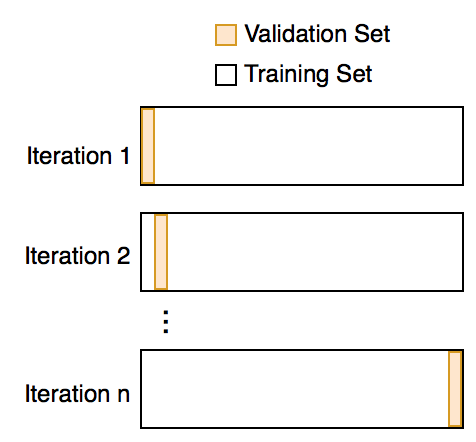
\includegraphics[width=.37\linewidth]{leave1.png}
  \caption{Leave-One-Out}
  \end{subfigure}
  \caption{Exhaustive cross-validation methods: Leave-p-Out (left) \& Leave-One-Out (right)}
  \label{fig:leavep}
\end{figure*}

\break\noindent\textbf{Non-exhaustive cross-validation}
\begin{itemize}
\item Holdout method \newline \index{holdout}
This method randomly splits the original data set into two sets being the training set and the test set. Usually, the test set is smaller than the training set so that the algorithm has more data to train on. This method involves a single run and so must be used carefully to avoid misleading results. It is therefore sometimes not considered a CV method \cite{kohavi1995study}.

\item $k$-fold\newline \index{k-fold}
This method randomly splits the original data set into $k$ equally sized subsets, as shown in Fig.~\ref{fig:kfold}. The function is then trained and validated $k$ times, each time taking a different subset as the test data and the remaining $(k-1)$ subsets as the training data, using each of the $k$ subsets as the test set once. The $k$ results are averaged to produce a single estimation. Stratified $k$-fold cross validation is a refinement of the $k$-fold method, which splits the original samples into equally sized and distributed subsets, having the same proportions of the different target labels \cite{kohavi1995study}.

\begin{figure}
\centering
  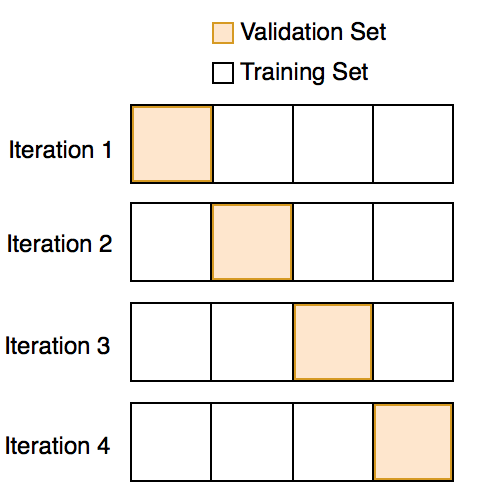
\includegraphics[width=0.5\linewidth]{kfold.png}
  \caption{$k$-Fold Cross Validation where $k$=4}
  \label{fig:kfold}
\end{figure}

\item Repeated random sub-sampling\newline \index{repeated random sub-sampling}
This method is also known as the Monte Carlo CV. It splits the data set randomly with replacement into training and test subsets using some predefined split percentage, for every run. Therefore, this generates new training and test data for each run but the test data of the different runs might contain repeated samples, unlike that of $k$-fold \cite{xu2001monte}.
\end{itemize}

All of the above cross-validation methods are used to check whether the model has been overfitted or underfitted and hence estimating the model's ability of fitting to independent data . Such ability is measured using quantitative metrics appropriate for the model and data \cite[-3\baselineskip]{kohavi1995study, arlot2010survey}. In the case of classification problems, the misclassification error rate is usually used whilst for regression problems, the mean squared error (MSE) is usually used. MSE is represented by Eq.~\ref{mse}, where n is the total number of test samples, $Y_i$ is the true value of the $i^{th}$ instance and $\hat{Y}_i$ is the predicted value of the $i^{th}$ instance.

\begin{equation}\label{mse}
MSE = \frac{1}{n}\sum^{n}_{i=1}(Y_i - \hat{Y}_i)^2
\end{equation}

Underfitting \index{underfitting} is when the model has a low degree (e.g. $y = x$, where the degree is 1) and so is not flexible enough to fit the data making the model have a low variance and high bias \cite{baumann2003cross}, as seen in Fig.~\ref{fig:models}a. Variance is the model's dependence on the training data and bias is model's assumption about the shape of the data \cite{arlot2010survey}. On the other hand, as seen in Fig.~\ref{fig:models}b, overfitting \index{overfitting} is when the model has a too high degree (e.g. $y = x^{30}$, where the degree is 30) causing it to exactly fit the data as well as the noise and so lacks the ability to generalize \cite{baumann2003cross}, making the model have a high variance. Cross-validation helps reduce this bias and variance since it uses most of the data for both fitting and testing and so helps the model learn the actual relationship within the data. This makes cross-validation a good technique for models to acquire a good bias-variance tradeoff \cite{arlot2010survey}.

\begin{figure*}
\centering
\begin{subfigure}
  \centering
  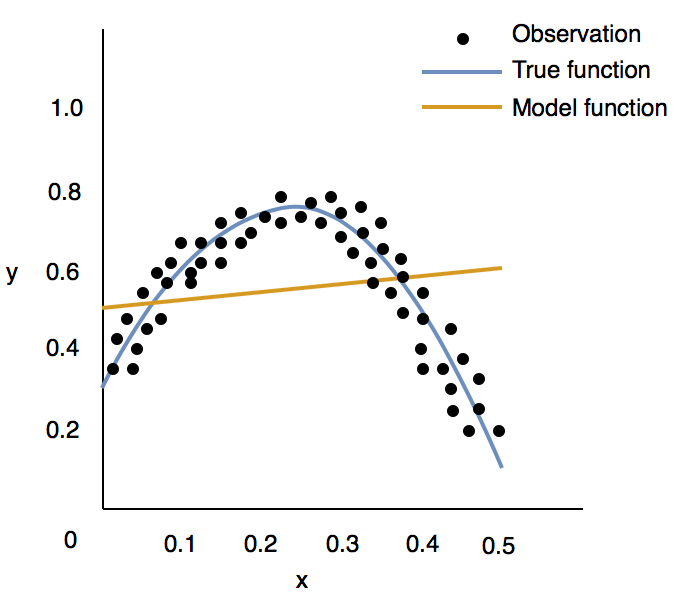
\includegraphics[width=0.4\linewidth]{underfitting.png}
  \caption{Underfitting}
  \label{fig:underfitting}
\end{subfigure}
\begin{subfigure}
  \centering
  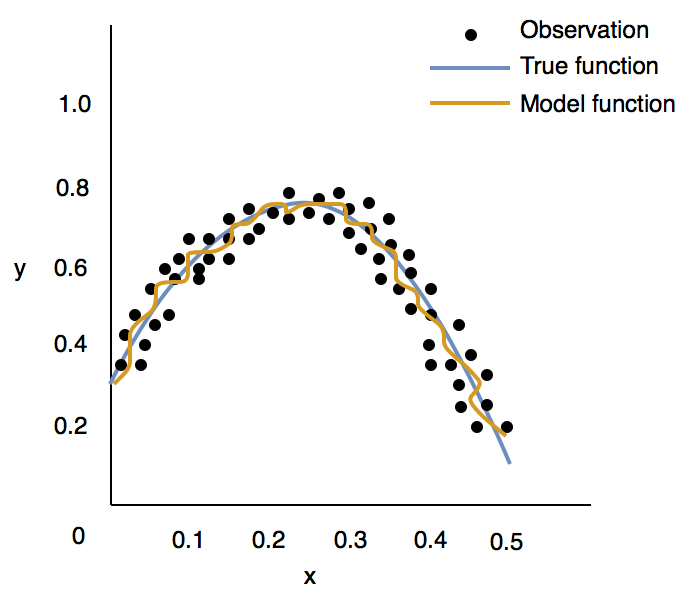
\includegraphics[width=.4\linewidth]{overfitting.png}
  \caption{Overfitting}
  \label{fig:overfitting}
\end{subfigure}
\caption{Underfitting (left) \& Overfitting (right)}
\label{fig:models}
\end{figure*}

As stated in \cite{Kohavi1995study}, the LOO method gives a 0\% accuracy on the test set when the number of target labels are equal to the number of instances in the dataset. It is shown that the $k$-fold CV method gives much better results, due to its lower variance, especially when $k = {10, 20}$. Furthermore, R. Kohavi et al. state that the best accuracy is achieved when using the stratified cross-validation method, since this has the least bias.

Therefore, lets take an example using the stratified $k$-fold cross-validation method with $k=10$. Let's say that we are trying to solve age group classification, using eight non-overlapping age groups being 0-5, 6-10, 11-20, 21-30, 31-40, 41-50, 51-60, and 61+. We are using the FG-NET labelled data set, which contains around 1000 images of individuals aged between 0 and 69. Before we can start training our model (e.g. CNN), we must divide our data set into training and test subsets and this is where cross validation comes in. Therefore, we start by taking the 1000 images of our data set and splitting them according to their target class. Let us assume we have an equal amount of 125 $(1000/8)$ images per class\footnote{Down-sampling or up-sampling are common techniques used when there is an unequal amount of samples for the different classes.}. As depicted in Fig.~\ref{fig:example}, we can now start forming our 10 folds by taking 10\% of each age-group bucket, randomly without replacement. Hence, we will end up with 10 subsets of 100 images that are equally distributed along all age-groups. With these subsets, we can estimate our model's accuracy with a lower bias-variance tradeoff. Since we are using 10-fold CV, we will train and test our model 10 times. For the first iteration, we shall use subset 1 as the validation set and subsets 2 to 10 as the training set, for the second iteration we use subset 2 as the test set and subsets 1 plus 3 to 10 as our training set, and so on (as shown in Fig.~\ref{fig:kfold}). For each iteration we use the misclassification error rate to obtain an accuracy value and we finally average the 10 accuracy rates to obtain the global accuracy of our model when solving age group classification, given the FG-NET data set. Hence, we have now estimated the prediction error of the model and have an idea of how well our model performs in solving such a problem. It is important to note that cross-validation is \textit{just} an estimation method and when using our model in real-life applications we do not apply CV but rather train our model with all the data we have.

\begin{figure*}
\centering
  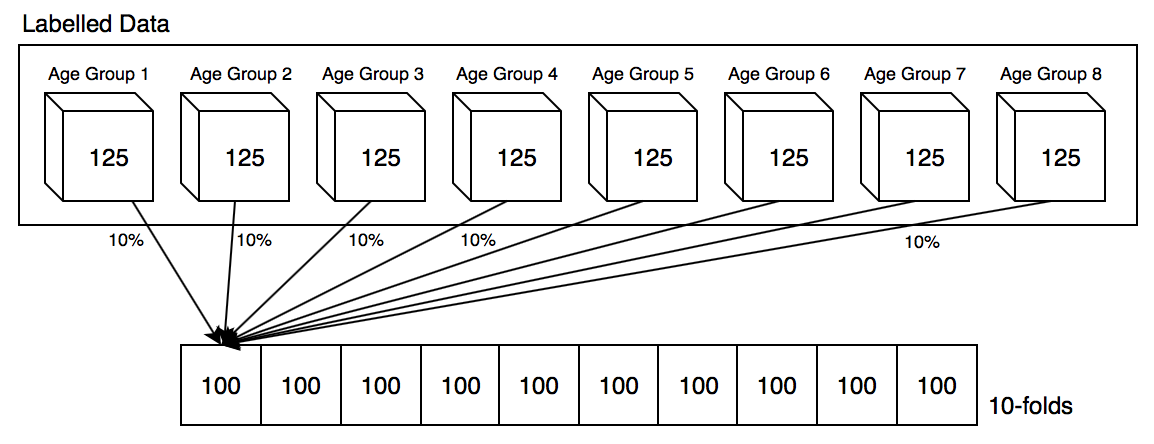
\includegraphics[width=0.88\linewidth]{example-cv.png}
  \caption{Stratified 10-fold cross-validation on 1000 labelled images of 8 different classes}
  \label{fig:example}
\end{figure*}

As concluded by \cite{varma2006bias}, cross-validation is well implemented when everything is taken place within every CV iteration (including preprocessing, feature-selection, learning new algorithm parameter values, etc.), and the least bias can be achieved when using nested CV methods.



\index{class options|)}
\chapter{Noise in datasets}
\label{ch:noiseindatasets}\index{noise in datasets|(}

As defined by \citet{hickey1996noise}, noise is anything that distorts the relationship between the describing attributes and the class.  Broadly speaking there are two types of noise: attribute (or feature) noise\index{noise in datasets!attribute noise} and class (or label) noise\index{noise in datasets!class noise} \citep{garcia2013, frenay2014classification}. In attribute noise, errors in one or more of the attributes that describe the class distort the true representation of the data.  Class noise on the other hand, is the mislabelling of instances in a dataset.  Missing observations can exist in both attributes and class, and are also considered as noise \citep{zhu2004class}.

The example dataset in Table~\ref{tab:noise_example} shows the various forms of noise. Instances \textit{5} and \textit{6} exhibit attribute noise, with instance \textit{5} having a missing value for attribute \textit{x\textsubscript{1}}, and instance \textit{6} having attribute \textit{x\textsubscript{2}} erroneously marked as \textit{c}. Instances \textit{1}, \textit{2}, \textit{4} and \textit{7} exhibit class noise.  Instance \textit{1} was mislabelled as \textit{0}, which should read \textit{1}.  Instances \textit{2} and \textit{4} are contradicting instances, implying that either one was mislabelled or the attribute readings were interpreted differently. Instance \textit{7} has a missing label.

\begin{margintable}
  \centering
  \fontfamily{ppl}\selectfont
  \begin{tabular}{cccc}
    \toprule
        \textit{\#} & \textit{x\textsubscript{1}} & \textit{x\textsubscript{2}} & \textit{Y} \\
    \midrule
    1 & a & d & \textcolor{red}{0} \\
    2 & a & c & \textcolor{red}{1} \\
    3 & b & c & 1 \\
    4 & a & c & \textcolor{red}{0} \\
    5 & \textcolor{red}{-} & d & 0 \\
    6 & b & \textcolor{red}{c} & 1 \\
    7 & b & d & \textcolor{red}{-} \\
    \bottomrule
  \end{tabular}
  \caption{A sample from a noisy dataset. \textit{Note: Noise is marked in red for ease of demonstration.}}
  \label{tab:noise_example}
\end{margintable}


Attribute noise is normally introduced through errors in the data collection or data processing stages, but also by corruption whilst the data are stored or transported \citep{garcia2013}.  Class noise on the other hand can be introduced through \citep{frenay2014classification}:
\begin{itemize}[-]
	\setlength{\itemsep}{0pt}
  	\setlength{\parskip}{0pt}
  	\setlength{\parsep}{0pt}
	\item insufficient information when labelling the instances;
	\item expert labelling errors; 
	\item subjectivity of the classes (for example in the case of medical diagnosis where experts can classify differently);
	\item encoding and communication problems; and
	\item using a cheap labelling method (such as non-expert or automated approaches). 
\end{itemize}

Unfortunately, noise is very common since reliable, noise free data are expensive and time consuming to obtain \citep{frenay2014classification}. The typical error rate in a dataset is 5\%. \citep{zhu2004class}. 


\section{Effects of noise}\label{sec:noise_effects}\index{noise in datasets!effects}

When learning a concept, algorithms assume and expect a correct and perfectly labelled dataset \citep{frenay2014comprehensive}.  Primarily, the noise in the training set reduces the predictive ability of the inferred model \citep{garcia2013, frenay2014comprehensive, frenay2014classification}. This can be seen in Figure~\ref{fig:noise_models} that shows the effect of noise on the classification accuracy of various classifiers.

\begin{figure}
  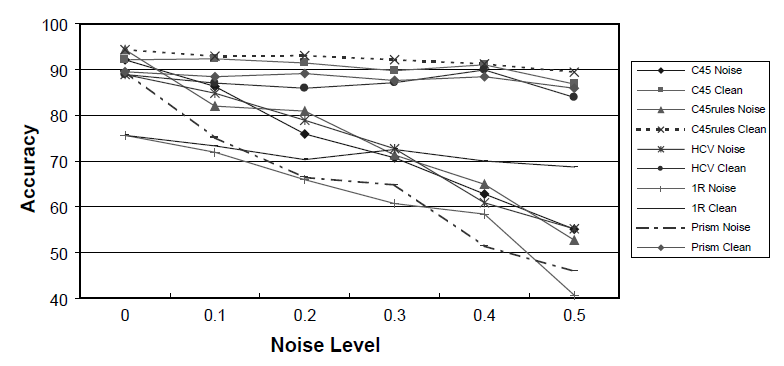
\includegraphics{graphics/noise_in_datasets/noise_models.png}
  \caption{A graph showing the effect of noise on the classification accuracy of various classifiers. Each model was trained on a noisy dataset and on a manually cleaned dataset. These are represented as \textit{XXX Noise} and \textit{XXX Clean} respectively, where \textit{XXX} denotes the classifier in question \citep{zhu2004class}.}
  \label{fig:noise_models}
\end{figure}

The extent of the damage caused by noise depends on various factors.  Class noise\index{noise in datasets!class noise} has been found to be more harmful than attribute noise\index{noise in datasets!attribute noise} \citep{zhu2004class}.  The reason for this is that whilst an attribute shares the predictive capability with other attributes, there is only one label and errors confuse the learning algorithm  \citep{zhu2004class}. 

\citet{zhu2004class} also found that not all attributes are equal in predicting the class and noise in the more important features are more damaging than others. The authors found that the higher the correlation between attribute and class the greater the impact of noise in the attribute.

Learning from a noisy dataset requires a larger training set \citep{frenay2014comprehensive, frenay2014classification} and is usually lengthier \citep{garcia2013}. Another cost of noise is the higher complexity of the inferred model \citep{garcia2013, frenay2014comprehensive, frenay2014classification}.

\section{Dealing with noise}\label{sec:noise_dealing}

To improve the performance of the inferred model, the effect of noise must be minimised \citep{zhu2004class}. There are various ways addressed in literature by which one can minimise such effects, which can be broadly classified into two categories: (i) improving the quality of the dataset (i.e. cleansing noise); and (ii) building models that are robust to noise.

\subsection{Cleansing noise}\label{sec:noise_cleansing}\index{noise in datasets!cleansing}

Noise is usually identified by a domain expert since automatic noise identification is difficult \citep{garcia2013}.  However, a domain expert is not always available and manual identification of noise is a lengthy process, therefore automated noise identification techniques are needed that either correct the noisy data or eliminate it. 

One cannot identify noise without making assumptions \citep{frenay2014classification}. Techniques that filter out noise remove instances that appear mislabelled or that disproportionately increase the model complexity \citep{frenay2014comprehensive}.  In some cases a classifier (noise filter) is trained to identify noisy instances. Other techniques aim at correcting errors or imputing missing values \citep{zhu2004class}.

For class noise\index{noise in datasets!class noise}, filtering out instances that appear noisy was found to improve results, but in the case of attribute noise\index{noise in datasets!attribute noise}, removing an instance for a noisy (including missing) attribute would not make sense, especially since other attributes may contain information that is useful for learning \citep{zhu2004class}. Instead, correcting or imputing the values was found to achieve better results. Techniques that deal with class noise include \textit{ensemble filters}, \textit{cross-validated committees filters} and \textit{iterative-partitioning filters} \citep{garcia2015data}.

Ensemble filters\index{noise in datasets!ensemble filters} aim to identify and remove mislabelled instances in the pre-processing phase \citep{garcia2015data, brodley1999identifying}. The filter consists of an ensemble of \textit{m} different classifiers (for example a decision tree, a 1-NN and an SVM) that are trained on the training data to act as noise filters. The training data is split into \textit{n} parts and for each of the \textit{m} classifiers, \textit{n} different algorithms are trained. Each algorithm classifies one of the \textit{n} subsets after being trained on the remaining \textit{n-1} subsets. If the predicted class does not match the true class, the element is marked as potentially noisy. The results of each of the \textit{m} classifiers are then compared and a consensus whether an element is noisy is obtained through a voting scheme.  Elements deemed noisy are removed from the training data.

Cross-validated committees filters\index{noise in datasets!cross-validated committees filters} use an approach very similar to that of ensemble filters except that the ensemble is made up only of decision trees \citep{garcia2015data, verbaeten2003ensemble}. It uses k-fold cross-validation to split the training data and train the base classifiers. Once again the noisy elements are identified through a voting scheme and eliminated.

Iterative-partitioning filters\index{noise in datasets!iterative-partitioning filters} are used for cleaning large datasets \citep{garcia2015data}. The training data is partitioned into manageable parts and cleansed in iterations until a stopping criterion is met. The stopping criterion is normally the percentage of noise that is tolerated.

\begin{figure}
  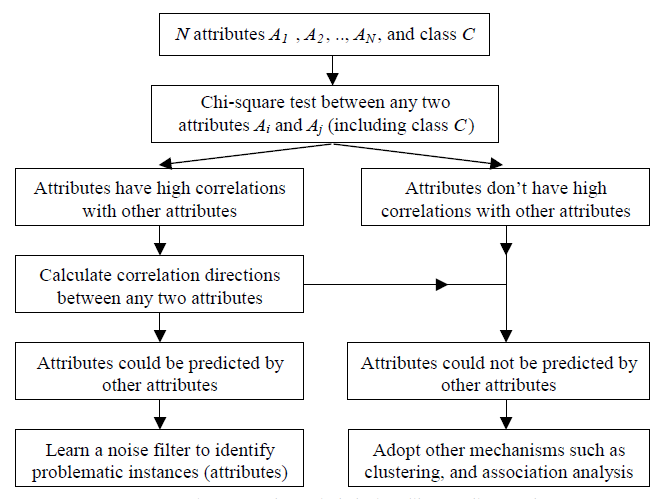
\includegraphics{graphics/noise_in_datasets/noise_imputation.png}
  \caption{The approach adopted by \citet{zhu2004class} to filter and correct attribute noise.}
  \label{fig:noise_imputation}
\end{figure}

Figure~\ref{fig:noise_imputation} depicts the approach taken by \citet{zhu2004class} to correct attribute noise\index{noise in datasets!attribute noise}, where for each attribute a strong correlation with other attributes is sought upon which noisy instances can be predicted (through a learning model) and corrected.  If a correlation is not found, corrections are based on other methods such as \textit{clustering} or \textit{k-nearest neighbour}.

The choice of noise filtering method should be based on the task at hand \citep{frenay2014classification}. The effectiveness of the noise filter should be evaluated on a dataset that is degraded with artificial noise\index{noise in datasets!artificial}.  The filtering precision can then be calculated through the number of correct instances that are filtered\index{noise in datasets!Type I errors} (\textit{Type I errors} - Equation~\ref{eq:noise_type1}) and the number of incorrect instances that are not filtered (\textit{Type II errors} - Equation~\ref{eq:noise_type2})\index{noise in datasets!Type II errors}.  These are calculated as follows: 

\begin{equation}\label{eq:noise_type1}
	ER\textsubscript{1} = \frac{\textnormal{\# of correctly labelled instances which are removed}}{\textnormal{\# of correctly labelled instances}}
\end{equation}

\begin{equation}\label{eq:noise_type2}
	ER\textsubscript{2} = \frac{\textnormal{\# of mislabelled instances which are not removed}}{\textnormal{\# of mislabelled instances}}
\end{equation}

Consequently, the \textit{Noise Elimination Precision} (NER)\index{noise in datasets!Noise Elimination Precision} can be calculated through Equation~\ref{eq:noise_ner} \citep{frenay2014classification}.

\begin{equation}\label{eq:noise_ner}
	NER = \frac{\textnormal{\# of mislabelled instances which are removed}}{\textnormal{\# of removed instances}}
\end{equation}

\subsection{Noise robust models}\label{sec:noise_robust_models}\index{noise in datasets!noise robust models}

No learning algorithm is immune to noise but some algorithms perform better than others in the presence of noise \citep{frenay2014comprehensive}.  \citet{kalapanidas2003machine} studied the noise sensitivity of ten different machine learning algorithms against various levels of artificially induced noise.  The results show that classifiers are much more noise tolerant than regressors.  The \textit{linear regression} algorithm proved to be the regressor least sensitive to noise, whilst the \textit{decision table classifier} proved to be the best performer overall.  A similar study \citep{nettleton2010study} found the \textit{na\"ive bayes} algorithm to be the most robust to noise.

\index{noise in datasets|)} 
\chapter{Online Learning Algorithms}
\label{ch:online-learning}\index{online-learning}

\section{Introduction}

\begin{figure}
  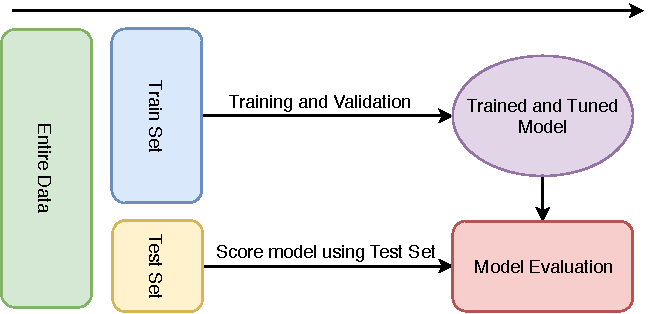
\includegraphics{online_learning/traditional.pdf}
  \caption{The traditional batch train-test machine learning approach workflow.}
  \label{fig:traditional_ml}
\end{figure}

In the traditional machine learning approach depicted in Figure~\ref{fig:traditional_ml}, we usually have some historical data to train an algorithm on for predicting some future events \citep{oza_online_2005}. However, since most data environments are dynamic and will change, the trained model eventually becomes outdated. To tackle this, we usually automate model re-training based on a timeframe (i.e.\ weekly or daily basis). Although this helps with keeping the model up-to-date, this is still not enough. Even if we consider model re-training on a daily basis, the model would still be at least one day late. 

Furthermore, as \citet{pagels_what_2018} argued, no matter how good a specific model is, it would always be an imperfect representation of the problem. Moreover, to have the best prediction for today, we cannot rely on a model with knowledge about yesterday only. Enter online learning algorithms, a family of techniques that are modelled to consume as much data available (one sample at a time), as fast as possible, while continuously learning and adapting different learning parameters. In the following sections, we will dive deeper into the subject of online learning, and its particular usage.

\begin{figure}
  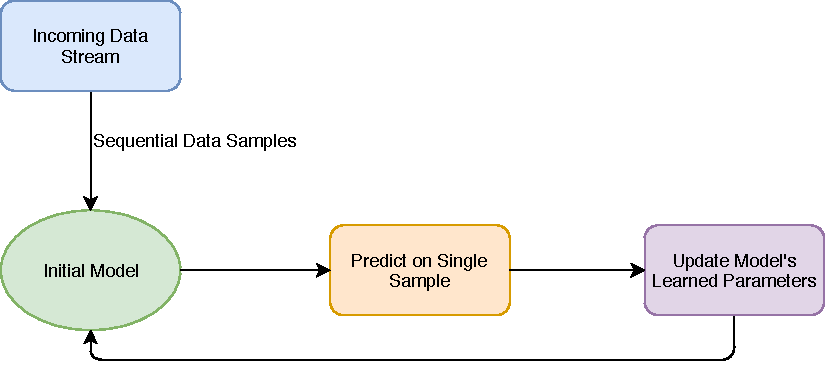
\includegraphics{online_learning/online.pdf}
  \caption{Basic workflow architecture of online learning.}
  \label{fig:online_ml}
\end{figure}

\section{Why use Online Learning?}

While being highly adaptable to dynamic underlying data structures since they make no statistical assumptions on the distribution of the data \citep{hoi_libol:_2014}, online learning techniques are also highly data efficient. Since online learning algorithms are only updated using the most recent data samples in the stream (as illustrated in figure~\ref{fig:online_ml}), such data samples are no longer stored or needed once the algorithm has passed over them, maintaining a much smaller data storage \citep{oza_online_2005}. Such algorithms are also very fast since only a single pass on a smaller data set is made, in contrast to the standard approach where the optimisation function needs multiple iterations over the entire dataset. Thus, as argued by \citet{hoi_online_2018}, online learning algorithms scale much better than the traditional approach.

As aforementioned, in offline machine learning, we load an entire dataset in memory, process it, then train a specific model, and then deploy the model into production. However, as more and more data is being generated, especially with the bright spotlight on Big Data, this methodology is proving to be more and more tedious. Some data sets are too large to fit into memory, even with distributed computing measures in place. Thus, online learning can drastically help in this scenario due to its small data storage property, especially when considered as online distributed computing and out-of-core computation \citep{zhang_projection-free_2017}, which is a huge plus.

To further extract the important usability of online learning, let us, as an analogy, consider the case of an online news portal where news articles are custom and shown to the users based on which categories that respective user usually tends to click. Pretending that a terrible disaster is happening or has happened on one specific day, and the government issues a 24-hour emergency evacuation; therefore, the majority of the user-base would start clicking on this news more and more. With the traditional batch approach, even with a re-training time of 24 hours, the system would fail to push this article to users who typically do not click on domestic affairs articles (i.e.\ users only interested in sports or entertainment). As a result, the same data content structure will be assumed by the algorithm even though there was a drastic change of events. 

In addition to this, given the same batch algorithm, after re-training in the following day, it would now start to suggest this article to a high percentage of the user-base, which by this time, such news might no longer be relevant or applicable.

Another small application resides in the online advertising domain. With different events and occasions happening every day, especially unscheduled or unforeseeable events which go viral, ads must stay relevant all the time to ensure the highest click-rate probability, and thus, must always synchronise to the affairs of the physical world. Ads must be intelligent enough to be aware of the hidden data distribution to adapt to data morphism.

In both examples, a traditional static model will fail due to being too slow to react to the dynamic underlying relationships present in the data. This problem is more formally known as concept drift \citep{schlimmer_incremental_1986}. The following section will further explain the notion of Concept Drift.

\section{Concept Drift}

Concept Drift occurs when the hidden context of the data changes. For instance, weather predictions are highly dependant on the season (the context), and as the seasons change so does the weather \citep{widmer_learning_1996}. As highlighted by \citet{krawczyk_online_2018, Gama2014ASO}, based on the distribution drift speed and severity, concept drift can be of four types as depicted in Figure~\ref{fig:cd}:

\begin{figure}
  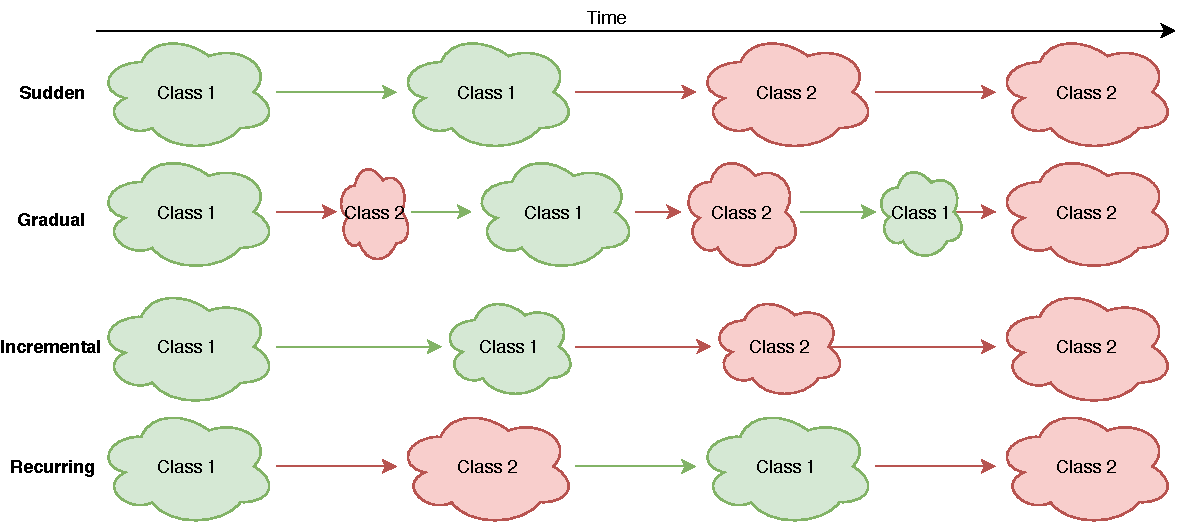
\includegraphics{online_learning/cd.pdf}
  \caption{The four types of Concept Drift.}
  \label{fig:cd}
\end{figure}

\begin{enumerate}
\item \textbf{Sudden:}
\textit{The data distribution is immediately changed to a different class.}
\item \textbf{Gradual:}
\textit{The data distribution gradually transitions by having varying proportions of the different classes mixing together over time, until it completely changes to the new class.}
\item \textbf{Incremental:}
\textit{The data distribution slowly morphs from one class to another.}
\item \textbf{Recurring:}
\textit{The data distribution periodically transitions between previous classes.}
\end{enumerate}

\subsection{Dealing with Concept Drift}

Thus, to combat this, as the concept drifts, so must the model's transition function that maps the inputs to the outputs. Due to the constant model updates performed through online learning (sample by sample), the transition function would be dynamic and adapts to the changing distribution \citep{Gama2014ASO, hoi_online_2018, Lane:1998:AOL:3000292.3000339}. In addition to this, another approach is to have a sliding window that shifts with the data stream. The purpose of this window, as discussed by \citet{wozniak_hybrid_2011}, is to keep a set of instances that offer the best representation of the present data distribution. As newer data samples arrive in the stream, the window slides towards more recent instances, resulting in the exclusion of the oldest samples from the window. Online learning achieves this window technique through the 'forgetting rate' which sets how fast older data is discarded to make room for newer instances. 

\subsection{Forgetting Rate}

Even though the design for most online learning algorithms is for fast execution speeds and thus adapted from less complex algorithms, implementation challenges are also present. As argued by \citet{gepperth_incremental_2016}, this leads us to one of the most significant problems in online learning, Catastrophic Interference. The latter happens when the model abruptly forgets knowledge learnt for previous data. Most online learning algorithms have a forgetting rate parameter. This parameter allows the user to decide the speed at which the learning algorithm forgets old data; thus, how much data to retain. Moreover, the correct calibration of this rate is essential and challenging to perfect since a high value would result in catastrophic interference, while a lower value would result in the algorithm not adapting to the incoming samples in the stream. In addition to this, good initialisations are critical in this approach to steer away from slow convergence.

\section{Conclusion}

In this chapter, we introduced and discussed the sub-field of online learning algorithms concerning machine learning. Online learning is a highly useful tool that allows us to take machine learning to a whole other level by solving problems that otherwise would seem to be out of our technical ability. With the exponential importance for Big Data analytics, online learning arms us with the capabilities to process high-velocity data while also being fast to adapt to frequent changes in the data due to the ever-increasing data velocity. %TODO


%%
% The back matter contains appendices, bibliographies, indices, glossaries, etc.

\backmatter

\bibliography{terms/noiseindatasets_is,terms/onlinelearning_df,terms/crossvalidation_lmd,terms/confusionmatrix_df,terms/activationfunctions_km} %TODO
\bibliographystyle{plainnat}

\printindex

\end{document}
